\subsubsection{Intel Xeon X5670}
In this section we analyze the behaviour of Sorting Algorithms on a Chip MultiProcessor (CMP), namely a Symmetric MultiProcessor (SMP) on chip. The CMP in question is the Intel Xeon X5670, described in~\ref{PCM}, which is a generic node of the cluster $PCM$. We will be able to test our algorithms for parallelism degrees up to 8. We expect that performance results on this architecture will be significantly different from the ones obtained on Pianosa, in particular from a \textit{qualitative} point of view. Indeed, there are two key factors: first, the huge amount of primary memory will diminish the overhead due to I/Os; second, the communications now take place in shared memory thus they are less expensive.

\begin{figure}[t]
	\begin{center}
		\includegraphics[scale=0.6]{plots/test_00_PCM/NxTxM/sequential_PCM_NxTxM}
	\end{center}
  	\caption{\textit{Intel Xeon X5670}. Completion Time for the Sequentialsort.}
  	\label{sequential-PCM}
\end{figure}

\paragraph{Scalability of Sorting Algorithms} Figure~\ref{PCM-NxTxM} and~\ref{PCM-MxTxN} show the time completion of Sorting Algorithms for data sets up to 2 GB. Exactly as on $Pianosa$, due to the fine grain computation, there is not any Sorting Algorithm that shows a good scalability for \textbf{small} data sets. On the other hand, the previous considerations on the primary memory size and the cost of communications justify intuitively why, for \textbf{large} data sets, most Sorting Algorithms scale better than on $Pianosa$ (even if still far away from the ideality). Figure~\ref{PCM-NxTxM} shows that increasing the parallelism degree from 2 to 4, a lot of Sorting Algorithms scale really close to the ideality, while from 4 to 8 there is still a gain, but in general lower. Exactly as on $Pianosa$, \textit{Bucketsort}, \textit{Samplesort} and \textit{Load-Balanced Multi-Way Mergesort} exhibit the best performance in terms of both scalability and time completion. \textit{Mergesort} (Figure~\ref{PCM-NxTxM-mergesort}) was bad on $Pianosa$ because of both the communications overhead and the unbalanced workload, but now exhibit a great scalability up to parallelism degree 8; this is thanks also to the faster hardware which let the last sequential phase of merging becoming less incisive on the overall time completion. Figure~\ref{PCM-NxTxM-quicksort} shows \textit{Quicksort} which has the worst performance TODO. Figure~\ref{PCM-NxTxM-kmerge} shows the bad performance of \textit{4-Way Mergesort}; this algorithm suffers the last phase of merging that, since it is made by a single process (see~\ref{kmerge}), becomes predominant with respect to the gain of the parallelization. 

\begin{figure}[h]
	\centering
	\subfloat[Quicksort.]{\label{PCM-NxTxM-sequential}\includegraphics[width=0.4\textwidth]{plots/test_00_PCM/NxTxM/quicksort_PCM_NxTxM}} 
	\hspace*{20pt}	
  	\subfloat[Bitonicsort.]{\label{PCM-NxTxM-bitonicsort}\includegraphics[width=0.4\textwidth]{plots/test_00_PCM/NxTxM/bitonicsort_PCM_NxTxM}} 
	
	\centering
	\subfloat[Bucketsort.]{\label{PCM-NxTxM-bucketsort}\includegraphics[width=0.4\textwidth]{plots/test_00_PCM/NxTxM/bucketsort_PCM_NxTxM}} 
  	\hspace*{20pt}
  	\subfloat[Samplesort.]{\label{PCM-NxTxM-samplesort}\includegraphics[width=0.4\textwidth]{plots/test_00_PCM/NxTxM/samplesort_PCM_NxTxM}} 
	
	\centering
  	\subfloat[Mergesort.]{\label{PCM-NxTxM-mergesort}\includegraphics[width=0.4\textwidth]{plots/test_00_PCM/NxTxM/mergesort_PCM_NxTxM}}   
  	\hspace*{20pt}  
  	\subfloat[4-Way Mergesort.]{\label{PCM-NxTxM-kmerge}\includegraphics[width=0.4\textwidth]{plots/test_00_PCM/NxTxM/kmerge_PCM_NxTxM}} 
	
	\centering
  	\subfloat[Load-Balanced Mergesort.]{\label{PCM-NxTxM-lbmergesort}\includegraphics[width=0.4\textwidth]{plots/test_00_PCM/NxTxM/lbmergesort_PCM_NxTxM}} 
  	\hspace*{20pt}  
  	\subfloat[Load-Balanced Multi-Way Mergesort.]{\label{PCM-NxTxM-lbkmergesort}\includegraphics[width=0.4\textwidth]{plots/test_00_PCM/NxTxM/lbkmergesort_PCM_NxTxM}} 	
  	
	\caption{\textit{Intel Xeon X5670}. Time Completion of Sorting Algorithms by varying the parallelism degree. Each shape on a graphic represents the Time Completion of a certain Sorting Algorithm for a data set of specific size.}
	\label{PCM-NxTxM}
\end{figure}
 
\begin{figure}[!ht]
	\centering
	\subfloat[Quicksort.]{\label{PCM-MxTxN-sequential}\includegraphics[width=0.4\textwidth]{plots/test_00_PCM/MxTxN/quicksort_PCM_MxTxN}} 
	\hspace*{20pt}	
  	\subfloat[Bitonicsort.]{\label{PCM-MxTxN-bitonicsort}\includegraphics[width=0.4\textwidth]{plots/test_00_PCM/MxTxN/bitonicsort_PCM_MxTxN}} 
  		
	\centering
	\subfloat[Bucketsort.]{\label{PCM-MxTxN-bucketsort}\includegraphics[width=0.4\textwidth]{plots/test_00_PCM/MxTxN/bucketsort_PCM_MxTxN}} 
  	\hspace*{20pt}
  	\subfloat[Samplesort.]{\label{PCM-MxTxN-samplesort}\includegraphics[width=0.4\textwidth]{plots/test_00_PCM/MxTxN/samplesort_PCM_MxTxN}} 
	
	\centering
  	\subfloat[Mergesort.]{\label{PCM-MxTxN-mergesort}\includegraphics[width=0.4\textwidth]{plots/test_00_PCM/MxTxN/mergesort_PCM_MxTxN}}   
  	\hspace*{20pt}  
  	\subfloat[4-Way Mergesort.]{\label{PCM-MxTxN-kmerge}\includegraphics[width=0.4\textwidth]{plots/test_00_PCM/MxTxN/kmerge_PCM_MxTxN}} 
	
	\centering
  	\subfloat[Load-Balanced Mergesort.]{\label{PCM-MxTxN-lbmergesort}\includegraphics[width=0.4\textwidth]{plots/test_00_PCM/MxTxN/lbmergesort_PCM_MxTxN}} 
  	\hspace*{20pt}  
  	\subfloat[Load-Balanced Multi-Way Mergesort.]{\label{PCM-MxTxN-lbkmergesort}\includegraphics[width=0.4\textwidth]{plots/test_00_PCM/MxTxN/lbkmergesort_PCM_MxTxN}} 
  	
	\caption{\textit{Intel Xeon X5670}. Time Completion of Sorting Algorithms for increasing sizes of the data set. }
	\label{PCM-MxTxN}
\end{figure} 


\paragraph{Comparison between Sorting Algorithms} Figures~\ref{PCM-NxTxA-small} and~\ref{PCM-NxTxA-large} highlight the behaviour of different Sorting Algorithms for specifics sizes of the data set. Notice an interesting aspect reguarding \textbf{small} data sets: we have seen that on $Pianosa$ best algorithms were \textit{qsort} and parallel \textit{Mergesort} (at low parallelism degrees). On this architecture things are deeply different and this is likely due to the fact that processes communications now take place in shared memory. Figure~\ref{PCM-NxTxA-small} shows that most of Sorting Algorithms, altough still far away from the linear scalability, definitely outperform \textit{qsort} (at least for sizes of the data set greater than 8 KB). Moreover, \textit{Mergesort} confirms itself as one of the best Sorting Algorithms both for small data sets and now even for \textbf{large} data sets, together with \textit{Bitonicsort}, \textit{Bucketsort}, \textit{Samplesort} and \textit{Load-Balanced (Multi-Way) Mergesort}.

\begin{figure}[!ht]
	\centering
	\subfloat[Data set of 1K integers.]{\label{PCM-NxTxA-1M}\includegraphics[width=0.4\textwidth]{plots/test_00_PCM/NxTxA/M1024_PCM_NxTxA}} 
	\hspace*{20pt}	
  	\subfloat[Data set of 2K integers.]{\label{PCM-NxTxA-2M}\includegraphics[width=0.4\textwidth]{plots/test_00_PCM/NxTxA/M2048_PCM_NxTxA}} 
  		
	\centering
	\subfloat[Data set of 4K integers.]{\label{PCM-NxTxA-4M}\includegraphics[width=0.4\textwidth]{plots/test_00_PCM/NxTxA/M4096_PCM_NxTxA}} 
  	\hspace*{20pt}
  	\subfloat[Data set of 8K integers.]{\label{PCM-NxTxA-8M}\includegraphics[width=0.4\textwidth]{plots/test_00_PCM/NxTxA/M8192_PCM_NxTxA}} 
	
	\centering
  	\subfloat[Data set of 16K integers.]{\label{PCM-NxTxA-16M}\includegraphics[width=0.4\textwidth]{plots/test_00_PCM/NxTxA/M16384_PCM_NxTxA}}   
  	\hspace*{20pt}  
  	\subfloat[Data set of 32K integers.]{\label{PCM-NxTxA-32M}\includegraphics[width=0.4\textwidth]{plots/test_00_PCM/NxTxA/M32768_PCM_NxTxA}} 
  	
	\centering
  	\subfloat[Data set of 64K integers.]{\label{PCM-NxTxA-16M}\includegraphics[width=0.4\textwidth]{plots/test_00_PCM/NxTxA/M65536_PCM_NxTxA}}   
  	\hspace*{20pt}  
  	\subfloat[Data set of 128K integers.]{\label{PCM-NxTxA-32M}\includegraphics[width=0.4\textwidth]{plots/test_00_PCM/NxTxA/M131072_PCM_NxTxA}}   	
  	
	%\caption{\textit{Intel Xeon X5670}. Time Completion for sorting \textit{small} data sets. Each graphic represents a data set of fixed size, while each shape on a graphic shows the Time Completion of a certain Sorting Algorithm for that data set.}
	%\label{PCM-NxTxA-small}
\end{figure} 

\begin{figure}[!ht]
	\ContinuedFloat
	\centering
	\subfloat[Data set of 256K integers.]{\label{PCM-NxTxA-1M}\includegraphics[width=0.4\textwidth]{plots/test_00_PCM/NxTxA/M262144_PCM_NxTxA}} 
	\hspace*{20pt}	
  	\subfloat[Data set of 512K integers.]{\label{PCM-NxTxA-2M}\includegraphics[width=0.4\textwidth]{plots/test_00_PCM/NxTxA/M524288_PCM_NxTxA}} 

	\centering
	\subfloat[Data set of 1M integers.]{\label{PCM-NxTxA-1M}\includegraphics[width=0.4\textwidth]{plots/test_00_PCM/NxTxA/M1048576_PCM_NxTxA}} 
	\hspace*{20pt}	
  	\subfloat[Data set of 2M integers.]{\label{PCM-NxTxA-2M}\includegraphics[width=0.4\textwidth]{plots/test_00_PCM/NxTxA/M2097152_PCM_NxTxA}} 
  		
	\centering
	\subfloat[Data set of 4M integers.]{\label{PCM-NxTxA-4M}\includegraphics[width=0.4\textwidth]{plots/test_00_PCM/NxTxA/M4194304_PCM_NxTxA}} 
  	\hspace*{20pt}
  	\subfloat[Data set of 8M integers.]{\label{PCM-NxTxA-8M}\includegraphics[width=0.4\textwidth]{plots/test_00_PCM/NxTxA/M8388608_PCM_NxTxA}} 
	
	\centering
  	\subfloat[Data set of 16M integers.]{\label{PCM-NxTxA-16M}\includegraphics[width=0.4\textwidth]{plots/test_00_PCM/NxTxA/M16777216_PCM_NxTxA}}   
  	\hspace*{20pt}  
  	\subfloat[Data set of 32M integers.]{\label{PCM-NxTxA-32M}\includegraphics[width=0.4\textwidth]{plots/test_00_PCM/NxTxA/M33554432_PCM_NxTxA}} 
  	
	\caption{\textit{Intel Xeon X5670}. Time Completion for sorting \textit{small} data sets. Each graphic represents a data set of fixed size, while each shape on a graphic shows the Time Completion of a certain Sorting Algorithm for that data set.}
	\label{PCM-NxTxA-small}
\end{figure} 

\begin{figure}[!ht]
	\centering
	\subfloat[Data set of 64M integers.]{\label{PCM-NxTxA-64M}\includegraphics[width=0.4\textwidth]{plots/test_00_PCM/NxTxA/M67108864_PCM_NxTxA}} 
	\hspace*{20pt}	
  	\subfloat[Data set of 128M integers.]{\label{PCM-NxTxA-128M}\includegraphics[width=0.4\textwidth]{plots/test_00_PCM/NxTxA/M134217728_PCM_NxTxA}} 
  		
	\centering
	\subfloat[Data set of 256M integers.]{\label{PCM-NxTxA-256M}\includegraphics[width=0.4\textwidth]{plots/test_00_PCM/NxTxA/M268435456_PCM_NxTxA}} 
  	\hspace*{20pt}
  	\subfloat[Data set of 512M integers.]{\label{PCM-NxTxA-512M}\includegraphics[width=0.4\textwidth]{plots/test_00_PCM/NxTxA/M536870912_PCM_NxTxA}} 
	
	\caption{\textit{Intel Xeon X5670}. Time Completion for sorting \textit{large} data sets. Each graphic represents a data set of fixed size, while each shape on a graphic shows the Time Completion of a certain Sorting Algorithm for that data set.}
	\label{PCM-NxTxA-large}
\end{figure} 

\begin{figure}[!ht]
	\centering
	\subfloat[Parallelism degree 2.]{\label{PCM-MxTxA-n2}\includegraphics[width=0.5\textwidth]{plots/test_00_PCM/MxTxA/n2_PCM_MxTxA}} 
	
	\centering
  	\subfloat[Parallelism degree 4.]{\label{PCM-MxTxA-n4}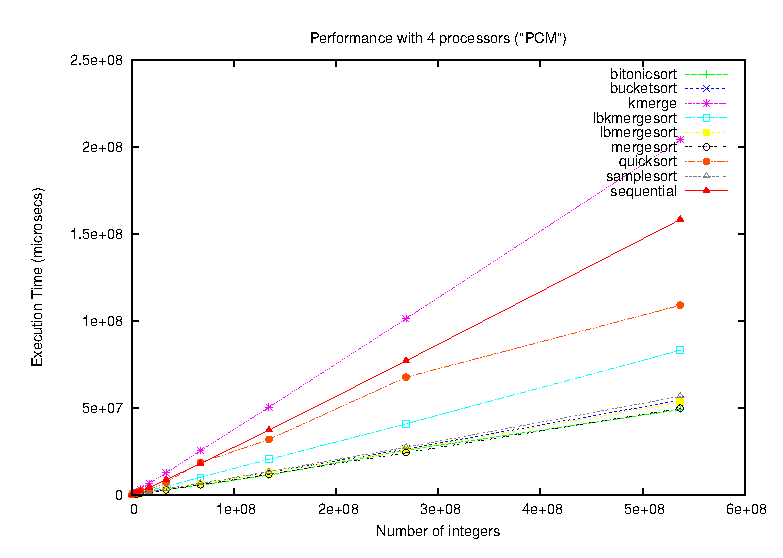
\includegraphics[width=0.5\textwidth]{plots/test_00_PCM/MxTxA/n4_PCM_MxTxA}} 
  		
	\centering
	\subfloat[Parallelism degree 8.]{\label{PCM-MxTxA-n8}\includegraphics[width=0.5\textwidth]{plots/test_00_PCM/MxTxA/n8_PCM_MxTxA}} 
  	
	\caption{\textit{Intel Xeon X5670}. Time Completion for sorting data sets with fixed parallelism degree.}
	\label{PCM-MxTxA}
\end{figure}

\clearpage
